\documentclass{../../../myassignment}

\exercisesheet{Oblig 4}{Optimalisering av FFT}
\courselabel{IN2060}
\usepackage{xfrac}
\usepackage{graphicx}

\begin{document}
	\subsection*{Core principle}
	Given the definition of a Fourier Transform: 
	$$ 
		F_k = \sum_{n=0}^{N-1} x_n * e^{-i\tau k \sfrac{n}{N}}
	$$

	we can see that this is equivalent to

	$$
		F_k = \sum_{n=0}^{\sfrac{N}{2}-1} x_{2m} * e^{-i\tau k \sfrac{2m}{N}} +  \sum_{n=0}^{\sfrac{N}{2}-1} x_{2m+1} * e^{-i\tau k \sfrac{2m+1}{N}}
	$$

	and with some simple algebra...
	$$
		F_k = \sum_{n=0}^{\sfrac{N}{2}-1} x_{2n} * \exp({-i\tau k \frac{n}{\sfrac{N}{2}}}) +  \sum_{n=0}^{\sfrac{N}{2}-1} x_{2n+1} * \exp({-i\tau k \frac{n+\sfrac{1}{2}}{\sfrac{N}{2}}})
	$$
	and with this follows something interesting. Both sum-loops include the same terms, except a +1/2 summand in the numerator, meaning we can make the following statement instead, bringing us to the next topic:
	\begin{align*}
		F_k &= \sum_{n=0}^{\sfrac{N}{2}-1} (x_{2n}\exp_{k,N}\cdot n) + \exp_k \sum_{n=0}^{\sfrac{N}{2}-1} (x_{2n+1}\exp_{k,N}\cdot n) \\
		\exp_{k,N} &= \exp(\frac{-i\cdot k\cdot\tau}{N})
	\end{align*}


	\subsection*{Twiddles}
	Due to the geometric representation of $\exp_{k,N}$, we know we have a periodic series of exponential values. This allows us to store \texttt{w\_out[i]} and \texttt{w\_out[i+N/2]} with the same, but complementary twiddle values. Since this halves the amount of work on not only the first iteration, but all of the iterations, we're really getting the time complexity down by doing this.
	
	Furthermore, since we are reusing many of the twiddle values in different parts of the recursion, these are needed over and over again. It is faster to only calculate them once, but for this we need to save the values somehwere. Since we only have 64 byte-lines, this is not going to hold. 32kB on L1 might hold if we're lucky, and 512kB is ``expectable''. Depending on the benchmarking values used, this will vary. Nevertheless, L2 access times are not the worst, so we can live with this, even if we only have 64 byte cache-lines, since hardware will (usually) prepare the next cache-line on-the-run for us, considering we travel in the same direction of the array. 


	\pagebreak
	\subsection*{Recursion}
	Recursion is evil! At least unnecessary recursion. 

	For each function call we're creating a new overheap and stack, which is slow. We would want to avoid this, unless we really need to. The main reason we want to avoid recursive calls is to use a whole cache-line at a time, and not have the processors jump back and forth between different memory addresses. When we can have a full cache-line full of values to use, this does not matter too much, and we can actually benefit from it, seeing as we have up to four available cores... but for all the smaller sections we should try something else instead. 

	A non-recursive implementation of the Discrete Fourier Transform is the trick here, and, note: we wouldn't really benefit from doing this on the whole initial sample array... as accessing all the samples takes a long time anyway. If we want to split this over multiple cores... yeah no. Bad idea, due to fake sharing of same memory sections. Nevertheless, as said, doing this on a sample size filling the whole cache-line? The processor really loves that.

	\subsection*{Other improvements}
	In the naive/original implementation, there were a bunch of calls to the heap. Four \texttt{malloc} calls per reursive function call. That's not a good idea, at all. Instead, let's make a buffer we can simply reuse. We don't even need to create one for the left side and another for the right, we can just use the memory address of the array, and assign \textit{it} to each recursive call instead. It needs half the sample size anyway, so that's perfect!

	Having two functions just to get the odd and even values of an array is highly unefficient. It can be done in one for-loop instead, already close-to-halving the time to do that. Besides, the overheap of having function calls is both slow and takes space.

	While \texttt{-O3} probably already does this, using bitshifting instead of halving/doubling is slightly faster due to how they are implemented on a hardware-level. Speaking of \texttt{-O3}... that's a nice flag to change. 

	\subsection*{Further improvements?}
	I have tried playing around with subthreading, but with little success. Using \texttt{\#pragma omp for schedule(dynamic, 64)} on some of the for-loops I would expect each thread to have access to its own chunks of arrays from \texttt{k,k+64 in range(0,iterations)}, and therefore not have any problems with sharing cache... but apparently I am not understanding this correctly. It only slows down my processes, so I have ommited it. The same applies for \texttt{pthread\_t}.

	Using subthreading for the first two nestings of the recursion is more likely than not a good idea, but I am yet to implement this. As it is now, \texttt{s\_out} would be shared over all the threads, which is not desirable as it is being used as a temporary cache. Potentially this could quadruple my timings, as the overheap of a few threads isn't a major issue... considering the compiler assumes the correct branch on the condition on whether or not to actually subthread or not. With a profile guided optimization this problem would cease to exist, though.

	\pagebreak
	\subsection*{Benchmarks}
	The following graphic is plotted from a Raspberry Pi 4B, since I didn't have any other device at hand, but we can still see some of the improvements over the naive implementation. The sudden jumps make it hard to actually make any meaningful conclusions, and a lack of x-values make it hard to see a growth.

	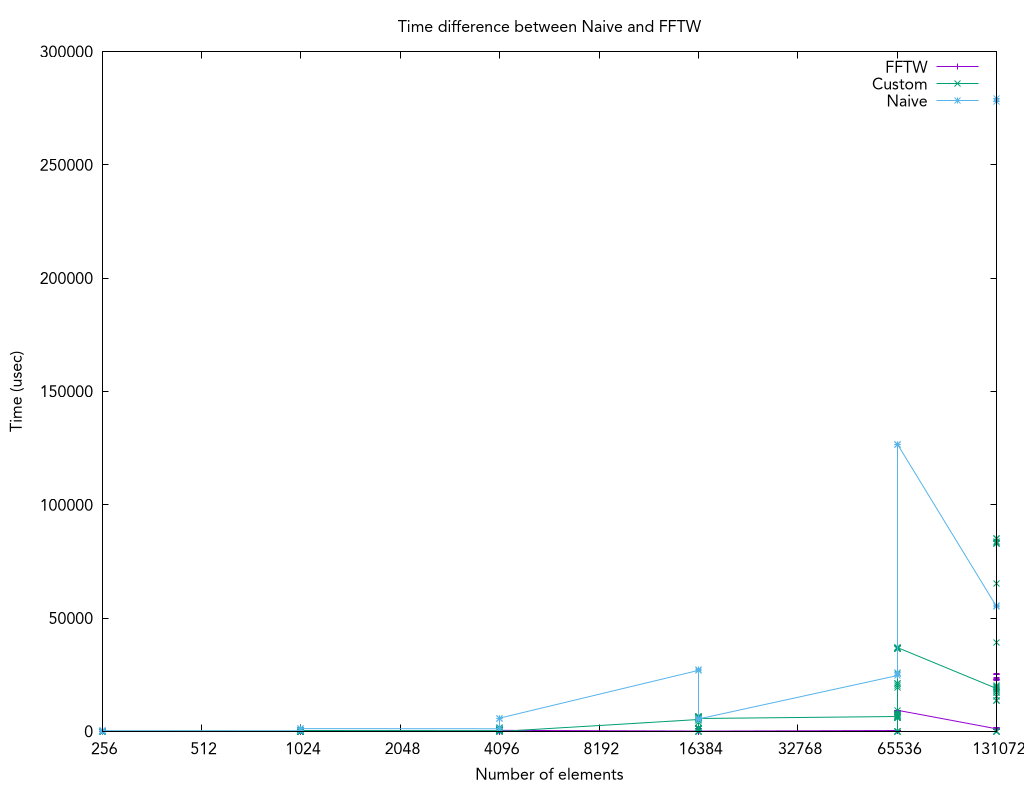
\includegraphics[width=0.7\textwidth]{img/diffs.png}

	A better view, including the old naive version, more values, and a logarithmic scale makes things better to visualize. We see there are some cases where the function just returns almost-nil. This must be investigated further. Nevertheless, it is clear we have a \texttt{O(n log n)} complexity. The pits we see at 256, 1024, 4096... are directly related to our line-cache.

	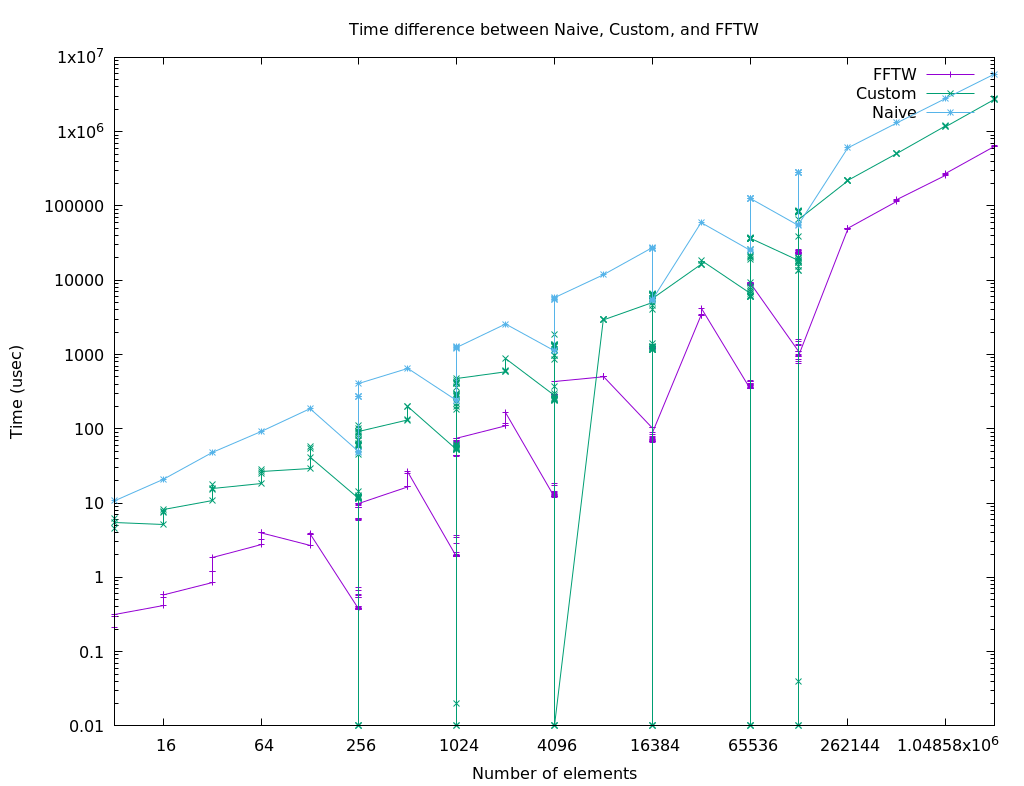
\includegraphics[width=0.85\textwidth]{img/better.png}

\end{document}